\documentclass{ctexart}
\title{股票交易大作业报告}
\author{陈启钰\,\,2300011447}
\date{\today}
\usepackage{geometry}
\usepackage{subfigure}
\usepackage{graphicx}
\usepackage{float}
\begin{document}
	\maketitle
	\newpage
	\section{海龟策略}
	\subsection{实现方法}
	先定义f1(p,$w$)函数为截取列表p的后$w$项(不够就返回p本身),然后定义aver函数计算列表p的各项平均值。
	
	第一天也就是列表ans的第零项为0,之后对于前$i+1$天可以先通过f1函数截取出一个列表,然后算出前$i$天的最大值和最小值,并于新列表的最后一项比较,在列表ans添加相应的操作。于是就可以实现\footnote{吐槽:这个列表项数从0开始真是个反人类设计}。
	\subsection{讨论}
	下面是四种不同初始资金条件下的买卖图(arg1=10)
	\begin{figure}[H]
		\centering
		\subfigure[poor]{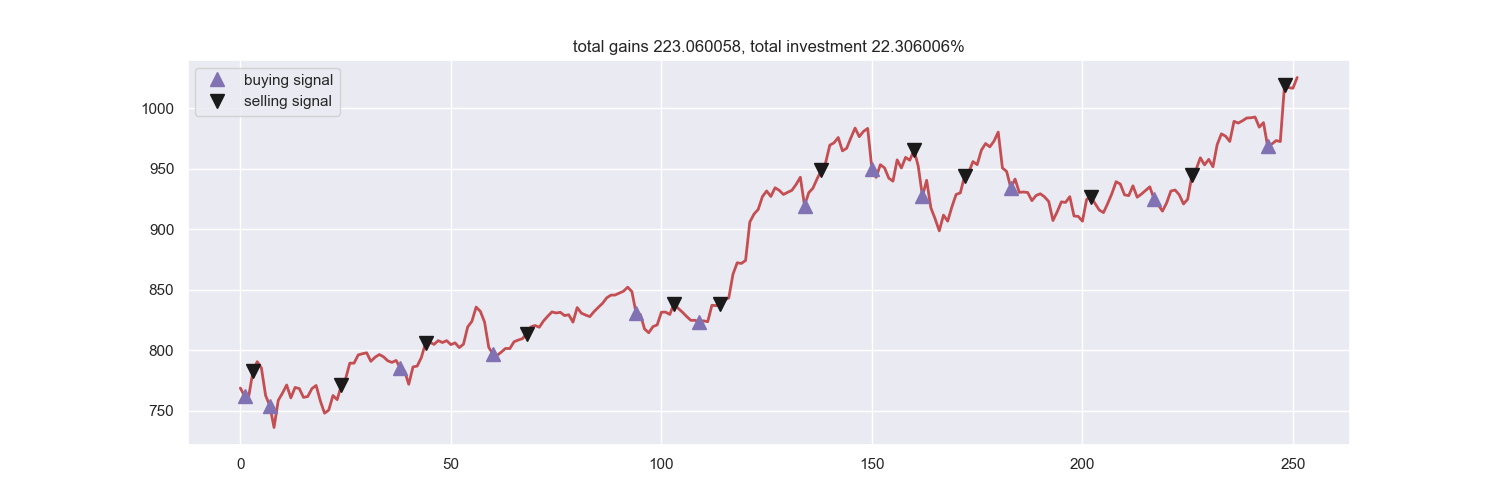
\includegraphics[width=13cm]{turtle_poor.png}}
	\end{figure}
	\begin{figure}[H]
		\centering
		\subfigure[normal]{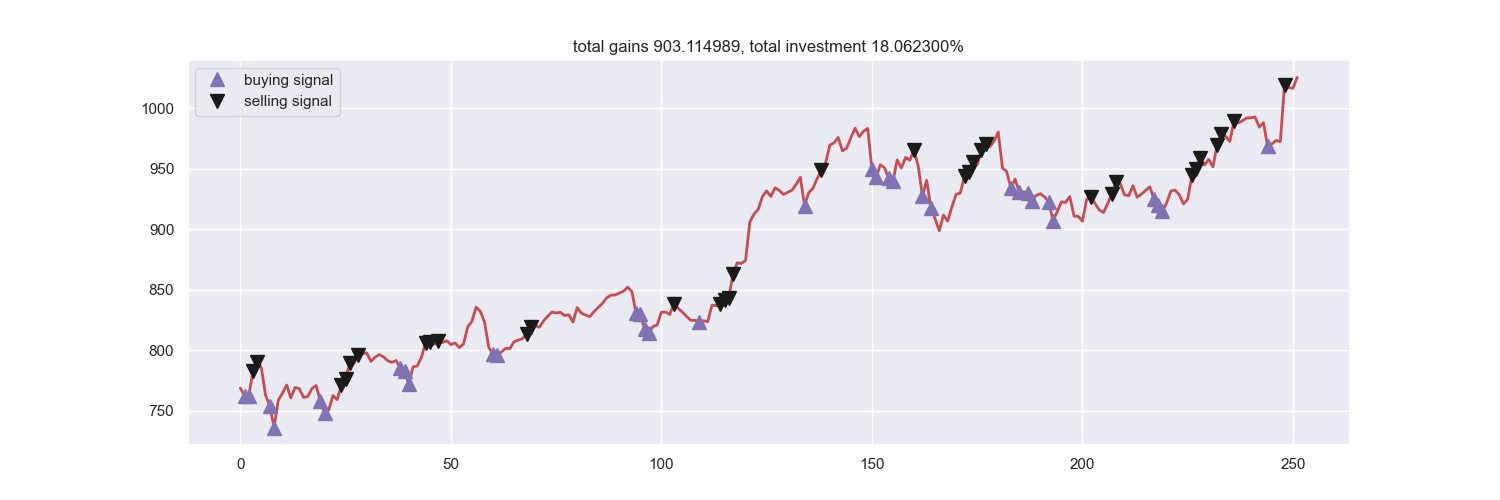
\includegraphics[width=13cm]{turtle_normal.png}}
	\end{figure}
	\begin{figure}[H]
		\centering
		\subfigure[rich]{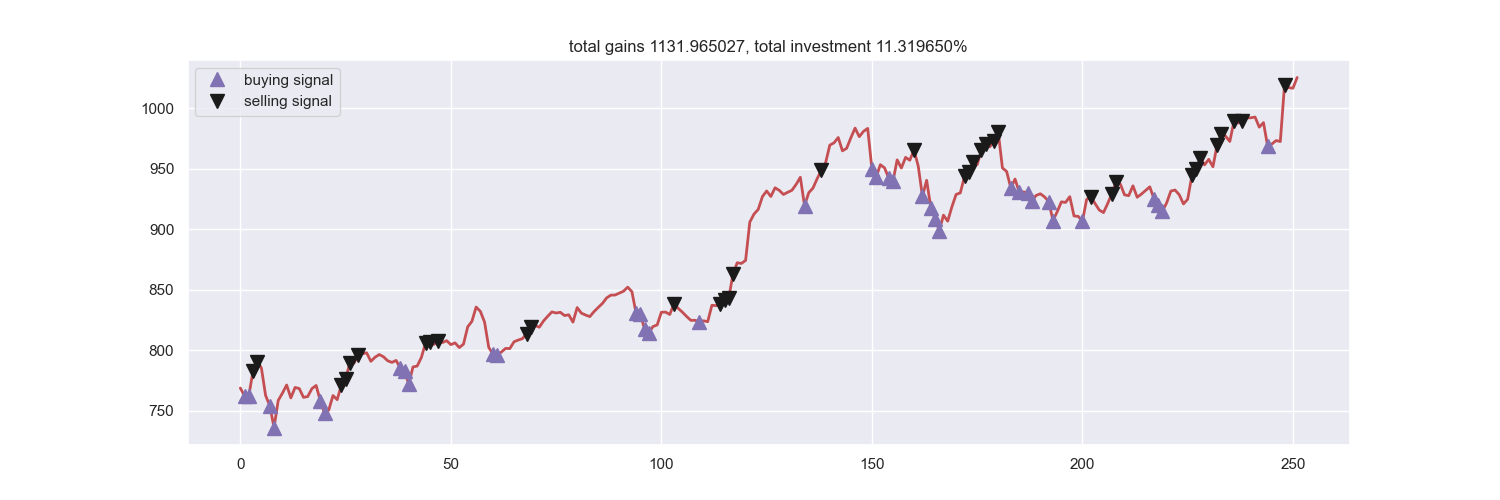
\includegraphics[width=13cm]{turtle_rich.png}}
	\end{figure}
	\begin{figure}[H]
		\centering
		\subfigure[inexhaustible]{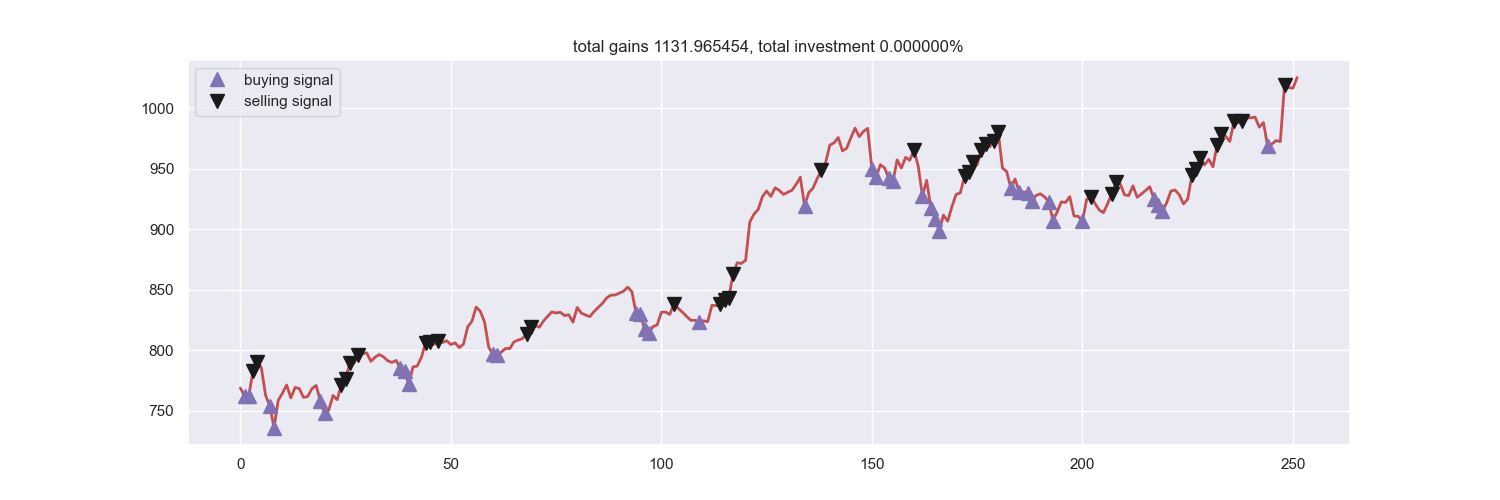
\includegraphics[width=13cm]{turtle_inexhaustible.png}}
		\caption{turtle策略的结果}
	\end{figure}
	通过观察四幅图片,目测感觉策略还是比较合理的,事实上也有盈利。在不同初始资金状况下,我们可以发现,资金越多,买卖越密集\footnote{有钱真好},而且资金少时的买卖在资金多时依然存在\footnote{这好像十分显然}。当然也有一个现象:资金多到一定程度时,利润固定了,比如rich和inexhaustible两种情况下利润相同。
	
	至于参数选取的影响,我只是发现当arg1大到一定程度的时候利润也是固定的,感性上来解释就是参考的天数越多了,大于最大值或者小于最小值就越难。我本来想在每种情况下绘制一张利润与参数选取的关系曲线,但是太复杂了,主要是数据无法批量生产,就很麻烦,于是放弃。
	\section{移动平均策略}
	\subsection{实现方法}
	movingaverage函数的编写:计算smat1、smat2、lmat1和lmat2,每一项的计算都可通过aver函数、f1函数和切片得到,aver(f1(price[0:i],w))表示的是price的前i项中的最后w项的平均值。然后通过比大小得到对应操作。
	\subsection{讨论}
	下面是四种不同初始资金条件下的买卖图(arg1=4,arg2=10)
	\begin{figure}[H]
		\centering
		\subfigure[poor]{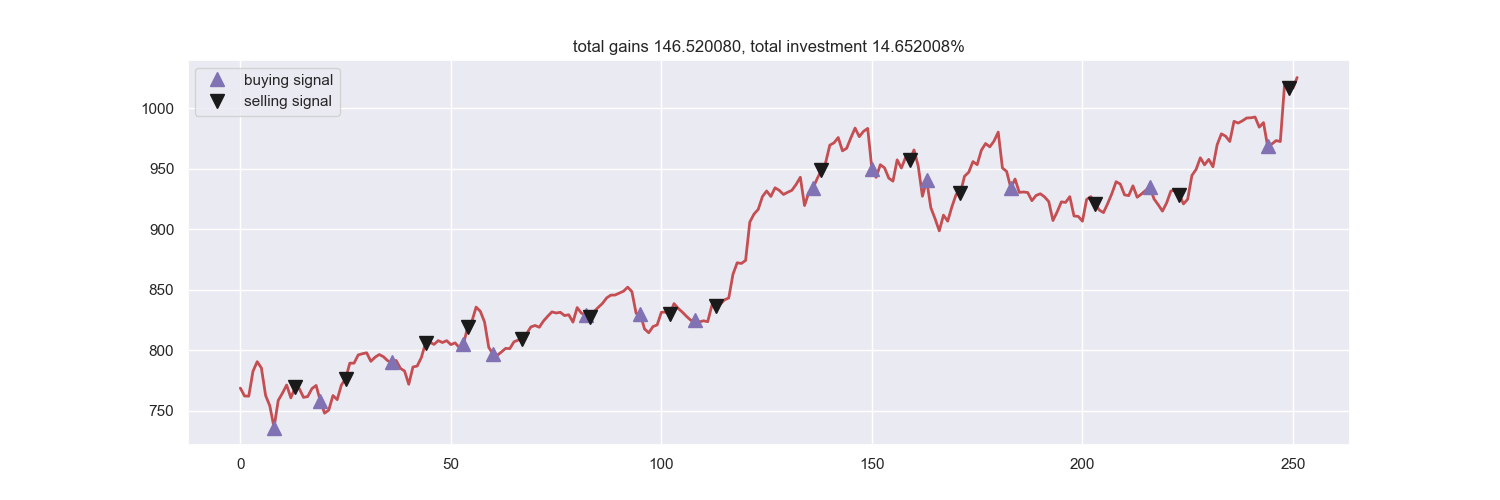
\includegraphics[width=13cm]{movingaverage_poor.png}}
	\end{figure}
	\begin{figure}[H]
		\centering
		\subfigure[normal]{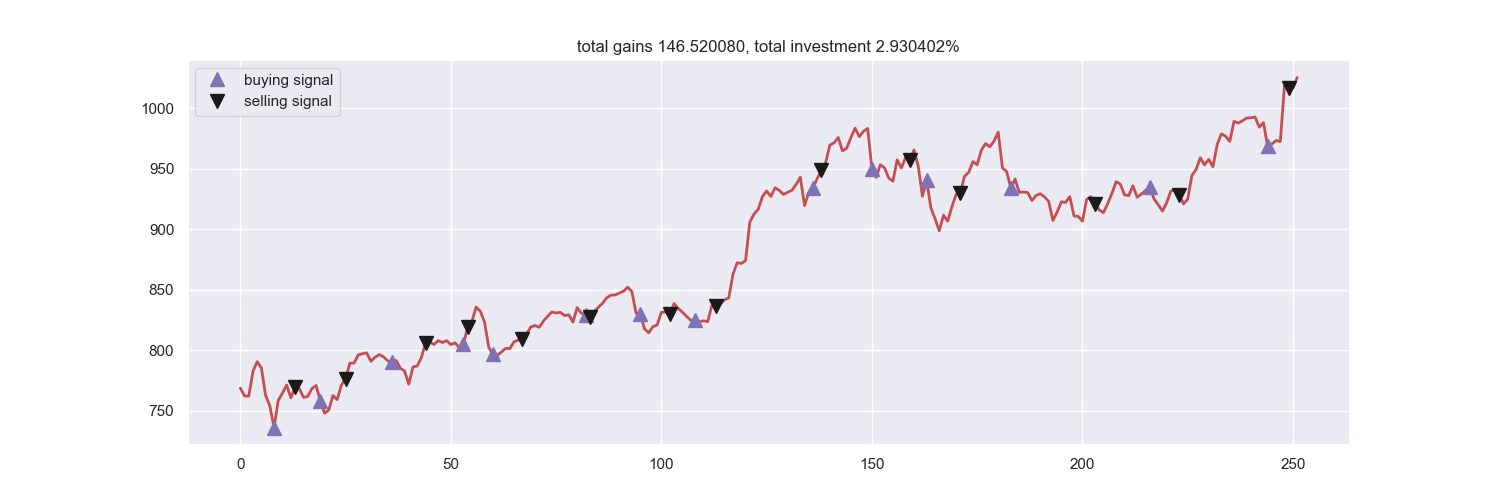
\includegraphics[width=13cm]{movingaverage_normal.png}}
	\end{figure}
	\begin{figure}[H]
		\centering
		\subfigure[rich]{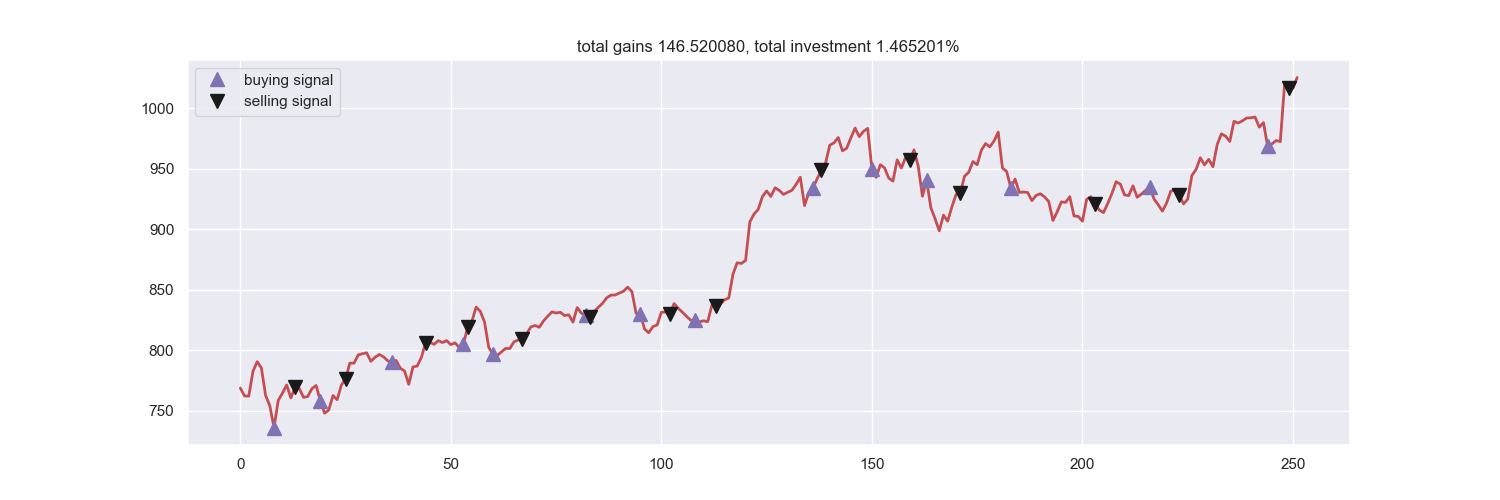
\includegraphics[width=13cm]{movingaverage_rich.png}}
	\end{figure}
	\begin{figure}[H]
		\centering
		\subfigure[inexhaustible]{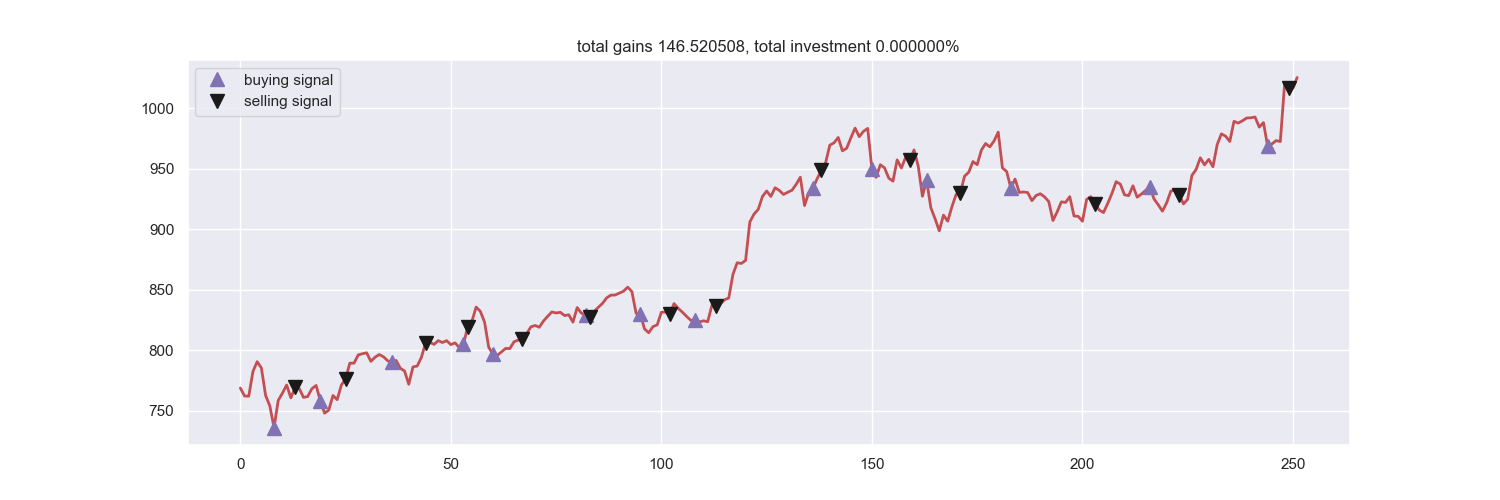
\includegraphics[width=13cm]{movingaverage_inexhaustible.png}}
		\caption{movingaverage策略的结果}
	\end{figure}
	观察结果发现,买卖总是交替的,也就是说一次买入以后下一次一定是卖出,再下一次一定是买入。通过短期平均曲线和长期平均曲线也可以分析出来这个结果,这是因为当短期平均超过长期平均以后下一次一定是长期平均超过短期平均。同时我们也可以得出结论:初始资金不会对movingaverage策略产生影响,只有两个参数会产生影响。
	\paragraph{注}这里我注意到如果按照README中的指示来执行的话,利润始终是负的,经过仔细思考,我觉得在短期平均超过长期平均的时候应该卖出而不是买入,同理长期平均超过短期平均的时候应该是买入,这个样子才能保证“价低买进价高卖出”,但是这好像涉及到了与计算概论无关的东西,不作讨论。相应的,我代码里面以及上述的四张图采用都是我的想法,如果一定要按照指示做的话,只需将strategy文件中的movingaverage函数中的ans.append()中的1和-1对调即可\footnote{还请助教手下留情【狗头】}。
	\section{abcd策略}
	\subsection{实现方法}
	f1函数和aver函数与移动平均策略相同,此外还定义了取交集函数jiaoji和集合减法函数jianfa。然后定义ma列表表示第$i$项之前的所有的平均(用到了f1和aver函数)。然后开始遍历abcd,根据要求,将满足条件的放入集合ABCD中。最后再判断每天应该进行的操作\footnote{说实话,我并没有看懂这个的原理是什么,当然如果我看懂了是不是就可以$\cdots$}。
	\subsection{讨论}
	下面是四种不同初始资金条件下的买卖图(arg1=20,arg2=5)
	\begin{figure}[H]
		\centering
		\subfigure[poor]{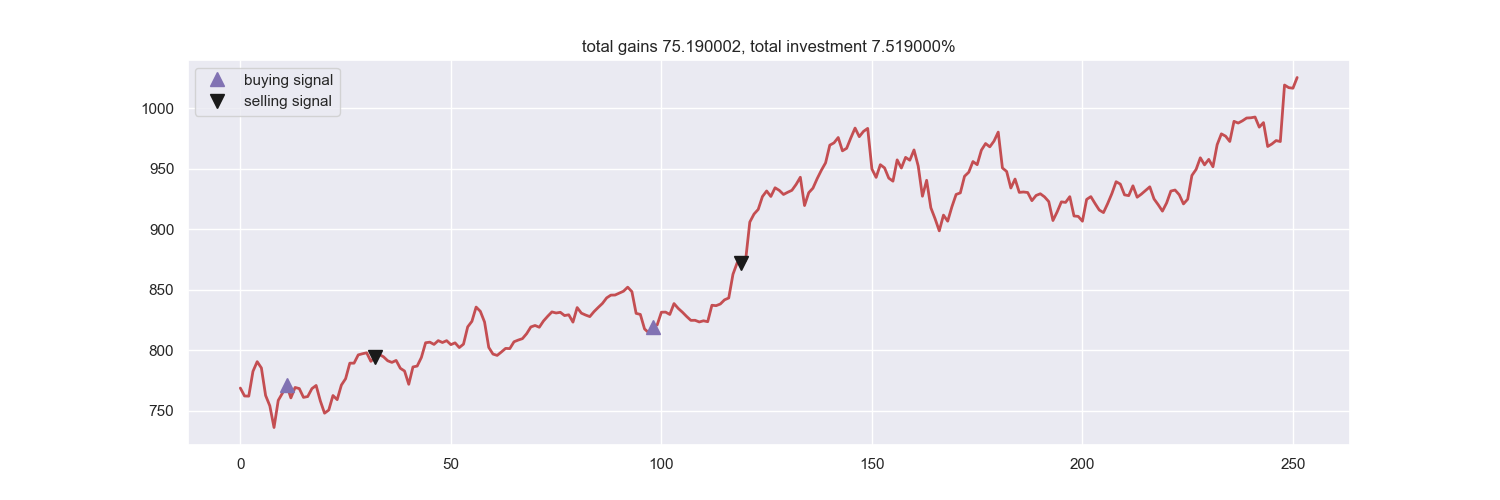
\includegraphics[width=13cm]{abcd_poor.png}}
	\end{figure}
	\begin{figure}[H]
		\centering
		\subfigure[normal]{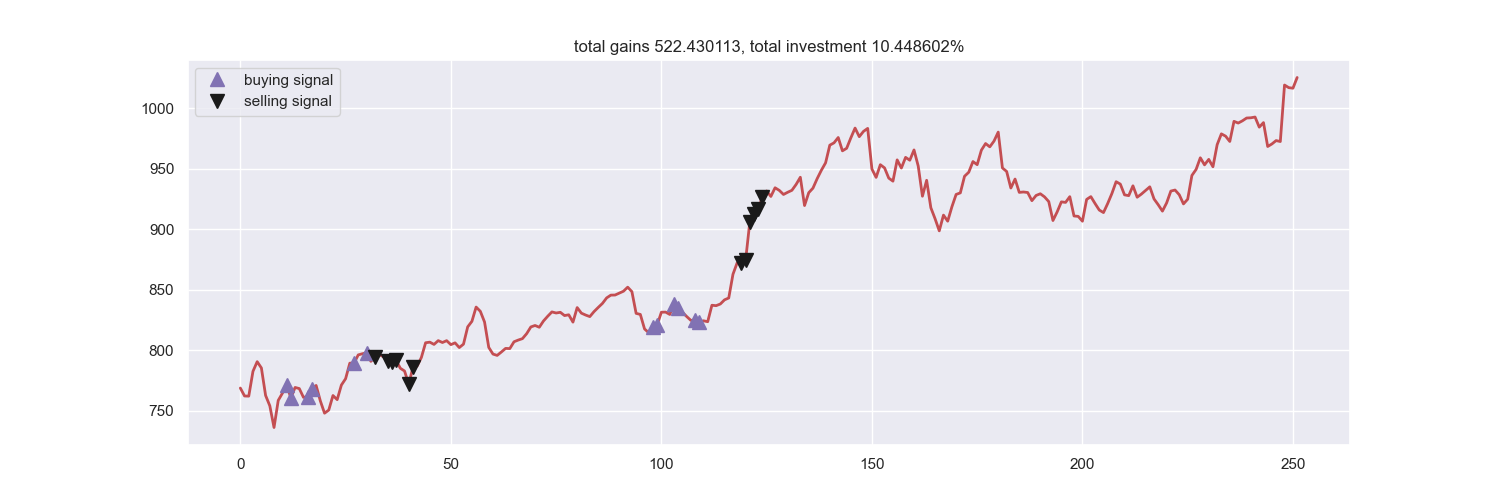
\includegraphics[width=13cm]{abcd_normal.png}}
	\end{figure}
	\begin{figure}[H]
		\centering
		\subfigure[rich]{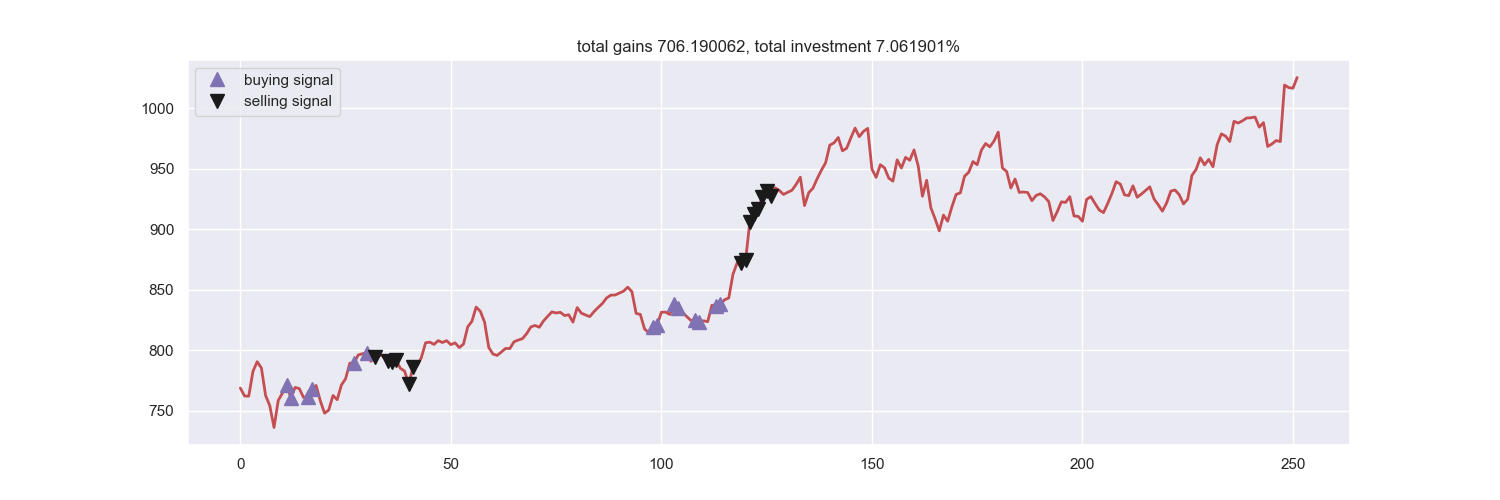
\includegraphics[width=13cm]{abcd_rich.png}}
	\end{figure}
	\begin{figure}[H]
		\centering
		\subfigure[inexhaustible]{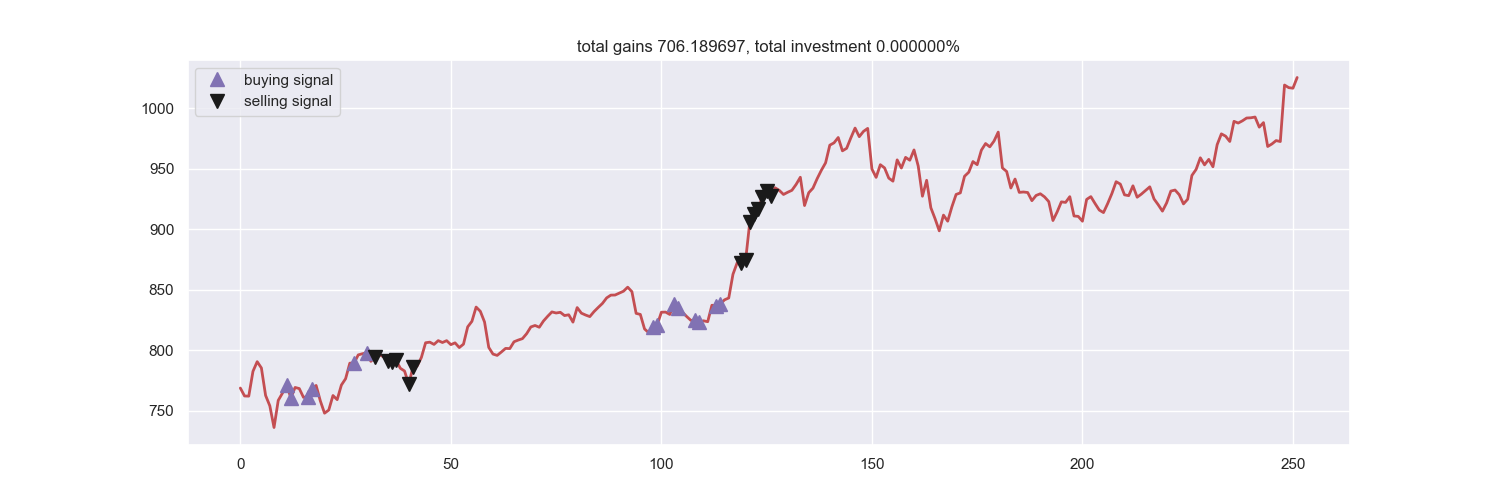
\includegraphics[width=13cm]{abcd_inexhaustible.png}}
		\caption{abcd策略的结果}
	\end{figure}
	依然,当初始资金多到了一定程度的时候,收益会到达一个稳定值,这是因为你永远可以在该买股票的时候买入。至于其它的规律...我是真找不出来了。
	\section{diy策略}
	\subsection{实现方法}
	我的diy策略主要是给定一个参数$w$,如果在$w$天内股价一直上升,就抛售,如果一直下降,就购入。代码也是显然的,其中judge1、judge2两个参数用来表征在$w$天内是否一直增加或减少。
	\subsection{讨论}
	下面是四种不同初始资金条件下的买卖图(arg1=3)
	\begin{figure}[H]
		\centering
		\subfigure[poor]{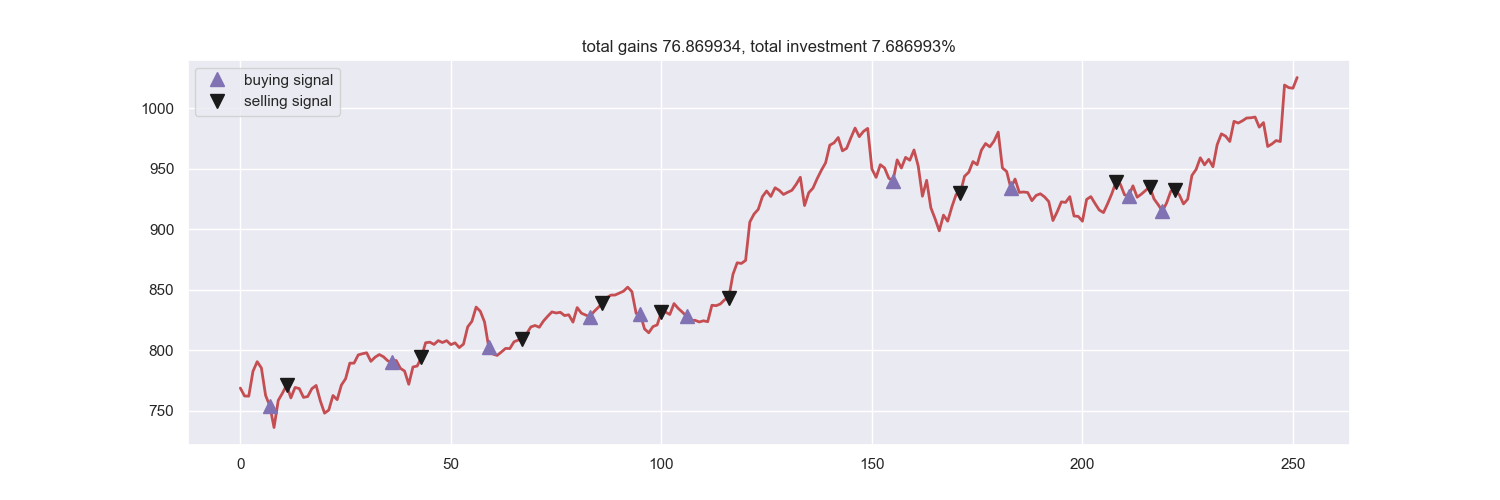
\includegraphics[width=13cm]{diy_poor.png}}
	\end{figure}
	\begin{figure}[H]
		\centering
		\subfigure[normal]{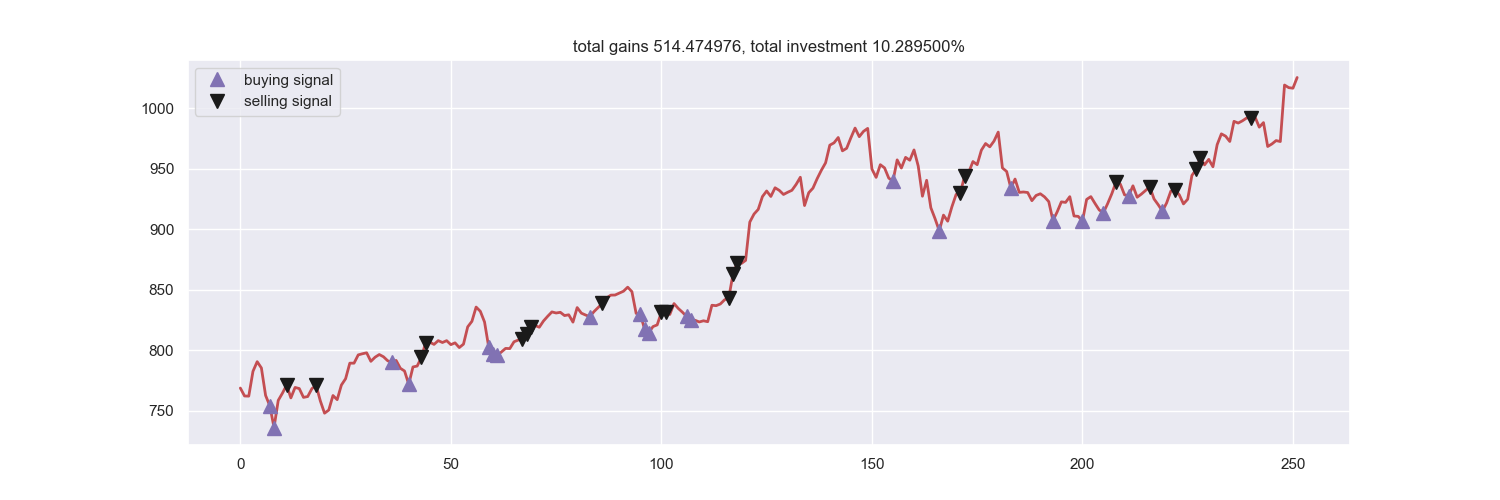
\includegraphics[width=13cm]{diy_normal.png}}
	\end{figure}
	\begin{figure}[H]
		\centering
		\subfigure[rich]{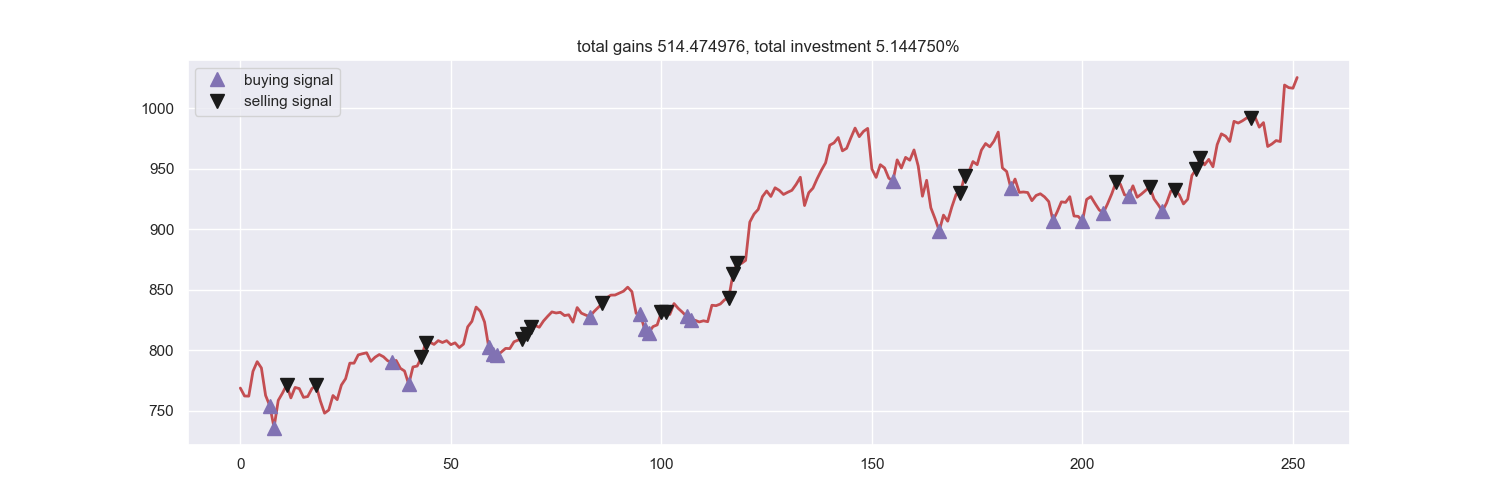
\includegraphics[width=13cm]{diy_rich.png}}
	\end{figure}
	\begin{figure}[H]
		\centering
		\subfigure[inexhaustible]{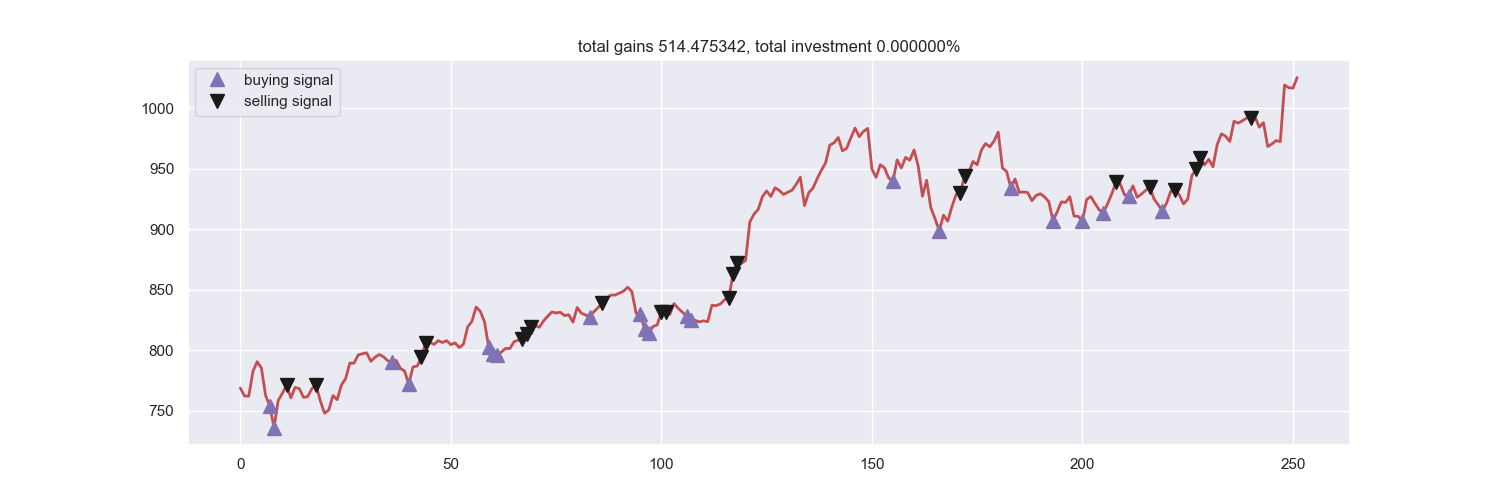
\includegraphics[width=13cm]{diy_inexhaustible.png}}
		\caption{diy策略的结果}
	\end{figure}
	观察可见,除poor情形外的其它三种情形行动相同,与前面相同。对于参数$w$的选取,显然不能过大,$w$过大会导致一个非常尴尬的结果就是股价单调减少或单调增加的条件很难满足,以至于最后不会有任何操作。当然,diy策略只是我的一个非常粗浅的愚蠢做法,真正炒股的时候肯定是去当炮灰的。
\end{document}